\chapter{Conclusion}
This chapter contains a short summary of our results and a conclusion to the research questions and topics discussed in Chapter~\ref{ch:discussion}. The final section gives suggestions on further work that can be done.

\section{Conclusion}
\begin{figure}[h!]
  \begin{subfigure}[b]{0.4\textwidth}
    \centering
    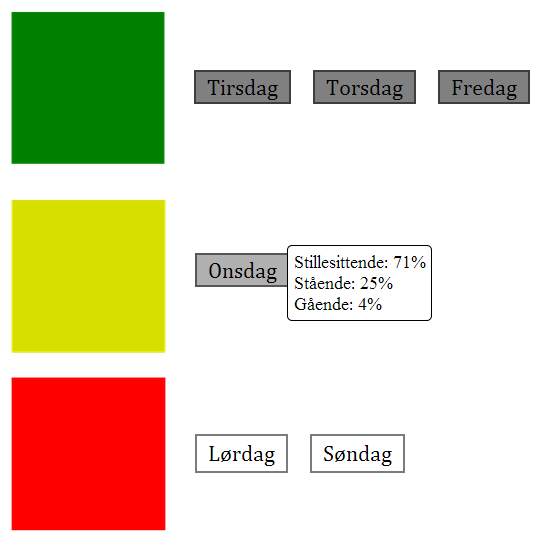
\includegraphics[width=\textwidth]{u1Second.png}
    \caption{U1}
  \end{subfigure} 
  \\
  \begin{subfigure}[b]{0.49\textwidth}
    \centering
    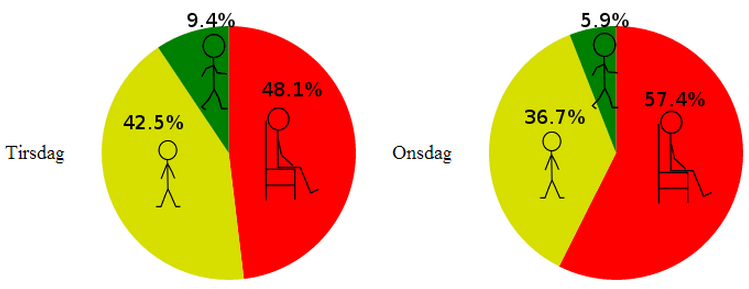
\includegraphics[width=\textwidth]{f1Second.png}
    \caption{F1}
  \end{subfigure} 
  \begin{subfigure}[b]{0.49\textwidth}
    \centering
    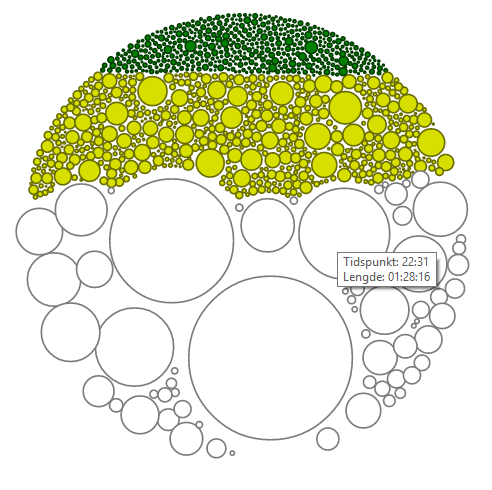
\includegraphics[width=0.5\textwidth]{f3Second.png}
    \caption{F3}
  \end{subfigure}
  \begin{subfigure}[b]{0.49\textwidth}
    \centering
    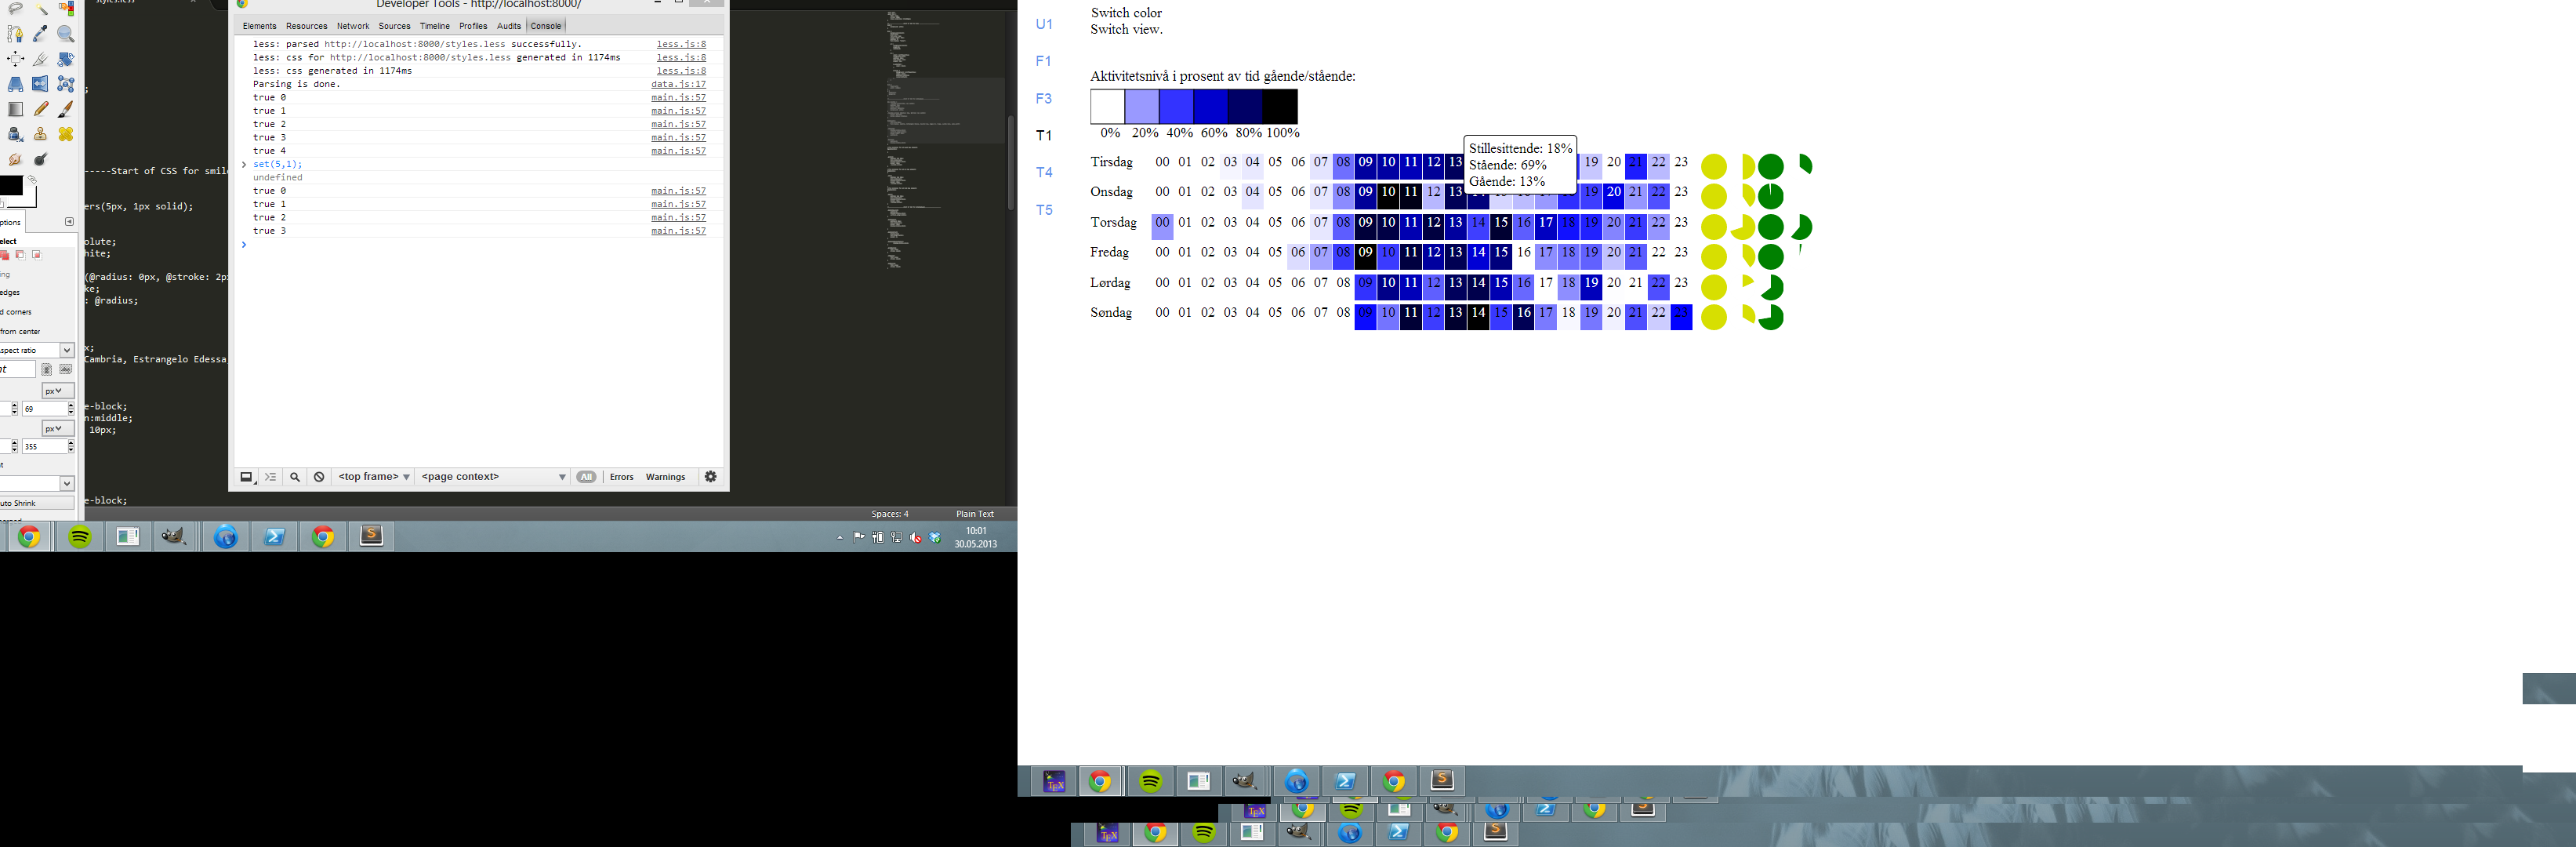
\includegraphics[width=\textwidth]{t1SecondWeek.png}
    \caption{T1}
  \end{subfigure} 
  \begin{subfigure}[b]{0.49\textwidth}
    \centering
    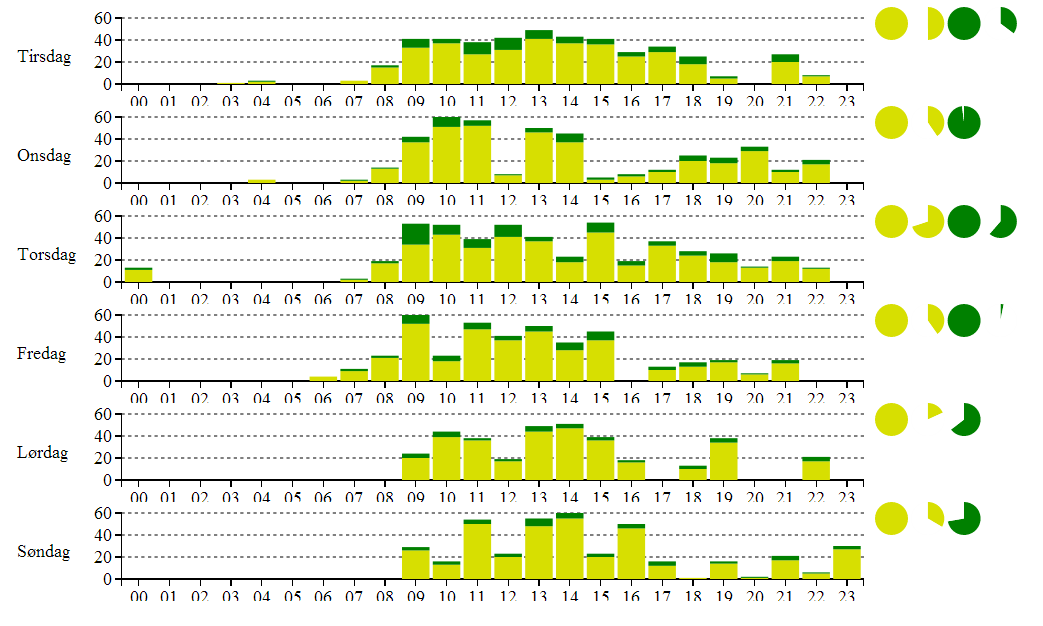
\includegraphics[width=\textwidth]{t5SecondWeek.png}
    \caption{T5}
  \end{subfigure}
  \caption[Accepted visualizations]{The five visualizations accepted by the participants of the second focus group.}
  \label{fig:visualizations}
\end{figure}

During the project we conducted two focus groups and created two prototype systems, see Chapters~\ref{ch:prototype1}--\ref{ch:focusGroup2}. These form the basis for most of our results. The first research question asked what types of scenarios physiotherapists saw as relevant when using visualizations to display quantitative data from sensors such as the activPAL. To answer this question we created a set of initial scenarios, as seen in Chapter~\ref{ch:initialRequirements}, by talking to a domain expert at St. Olav's Hospital. These initial scenarios were then discussed with the participants from the two consecutive focus groups to create five scenarios (see Table~\ref{tab:finalScenarios}.) that all the physiotherapists agreed upon.
\begin{table}[h!]
  \begin{tabular}{|c|p{10cm}|}
    \hline
    \textbf{Id} & \textbf{Scenario} \\ \hline
    S2-1 & When analysing patients activity level, either individually or in cooperation with occupational therapists or other physiotherapists. \\ \hline
    S2-2 & In consultation with the patient. \\ \hline
    S2-3 & In communication with nursing homes and home care personnel. \\ \hline
    S2-4 & In consultation with next of kin. \\ \hline
    S2-5 & For educational purposes. \\ \hline
  \end{tabular}
  \caption[Final scenarios]{Table showing the scenarios after the second focus group.}
  \label{tab:finalScenarios}
\end{table}

The second research question was concerned with the functional and \gls{ux} requirements for visualizations of data from sensors such as activPAL. The initial requirements were created after an interview with a domain expert at St. Olav's Hospital, see Chapter~\ref{ch:initialRequirements}. The requirements were then discussed and revised in the two focus groups, details can be found in Chapter~\ref{ch:focusGroup1} and~\ref{ch:focusGroup2}. The result after the two revision can be seen in Table~\ref{tab:f2ReqCon} and Table~\ref{tab:f2ReqUxCon}.

\begin{table}[h!]
  \begin{center}
  \begin{tabular}{|c|p{12cm}|}
    \hline
      \textbf{Id} & \textbf{Requirement} \\ \hline
    \multicolumn{2}{|l|}{The visualizations should \ldots} \\ \hline
      R2-1 & give the user an overview of the week where the days are classified by national recommendations or personal goals \\ \hline
      R2-2 & show the activity level for each hour of the day \\ \hline
      R2-3 & make it easy to identify the length of activity intervals \\ \hline
      R2-4 & make it possible to compare multiple days \\ \hline
      R2-5 & make it easy to identify hours of the day where activity can be added \\ \hline
      R2-6 & show the activity level compared to national or personal goals \\ \hline
      R2-7 & let the user identify patients that are active during the night \\ \hline
      R2-8 & let the user compare two separate weeks to see the patient's progress \\ \hline
      R2-9 & should be printable in grayscale \\ \hline
      R2-15 & show the activity distribution for a day (sedentary, standing, walking) \\ \hline
      R2-16 & allow the users to toggle if nighttime should be included or not \\ \hline
  \end{tabular}
  \end{center}
  \caption[Final functional requirements]{Functional requirements from the second focus group.}
  \label{tab:f2ReqCon}
\end{table}

\begin{table}[h!]
  \begin{center}
  \begin{tabular}{|c|p{12cm}|}
    \hline
      \textbf{Id} & \textbf{Requirement} \\ \hline
    \multicolumn{2}{|l|}{The visualizations should \ldots} \\ \hline
      F2-10 & not be judgemental towards the patient's activity level \\ \hline
      F2-11 & should be honest about the patient's activity level \\ \hline
      F2-12 & should motivate the patient to be more active \\ \hline
      F2-13 & should be intuitive and easy to understand for the user and third parties \\ \hline
      F2-14 & be easy to explain to cognitively capable patients \\ \hline
  \end{tabular}
  \end{center}
  \caption[Final user experience requirements]{User experience requirements from the second focus group.}
  \label{tab:f2ReqUxCon}
\end{table}

\clearpage

The third research question asked what types of visualizations would be preferred by the physiotherapists for the scenarios and requirements stated above. Two set of prototypes were created to answer this question, the five visualizations accepted by the physiotherapists can be seen in Figure~\ref{fig:visualizations}. The first prototype had a total of nine different visualizations, whereof four were discarded after the first focus group, see Chapter~\ref{ch:focusGroup1}. For the second focus group a new prototype was created using the feedback from the first focus group, as can be seen in Chapter~\ref{ch:prototype2}. The second prototype contained six visualizations, one was discarded after the second focus group. Time did not permit to create a new prototype using feedback from the second focus group, so not all of the requirements were covered by the visualizations. Table~\ref{tab:requirementsVisualizations} and Table~\ref{tab:scenarioVisualizations} show which visualizations satisfy which requirements and scenarios.

\begin{table}[h!]
  \centering
  \resizebox{\linewidth}{!}{
    \begin{tabular}{|c|c|c|c|c|c|c|c|c|c|c|c|}
      \hline
      & R2-1 & R2-2 & R2-3 & R2-4 & R2-5 & R2-6 & R2-7 & R2-8 & R2-9 & R2-15 & R2-16 \\ \hline
      U1 & + & -- & -- & + & -- & -- & -- & -- & + & -- & -- \\ \hline
      F1 & -- & -- & -- & + & -- & -- & -- & -- & + & + & -- \\ \hline
      F3 & -- & -- & + & -- & + & -- & -- & -- & -- & + & -- \\ \hline
      T1 & -- & + & -- & + & + & + & + & -- & -- & -- & -- \\ \hline
      T5 & -- & + & -- & + & + & + & + & -- & + & -- & -- \\ \hline
    \end{tabular}
  }
  \caption[Requirements and visualizations]{Table showing which requirements each visualization satisfies.}
  \label{tab:requirementsVisualizations}
\end{table} 

\begin{table}[h!]
  \centering
  \begin{tabular}{|c|c|c|c|c|c|}
    \hline
       & S2-1 & S2-2 & S2-3 & S2-4 & S2-5 \\ \hline
    U1 & +  & +  & -- & +  & +  \\ \hline
    F1 & +  & +  & +  & +  & +  \\ \hline
    F3 & +  & -- & +  & -- & +  \\ \hline
    T1 & +  & -- & +  & -- & +  \\ \hline
    T5 & +  & +  & +  & +  & +  \\ \hline
  \end{tabular}
  \caption[Scenarios and visualizations]{Table showing which scenarios each visualization satisfies.}
  \label{tab:scenarioVisualizations}
\end{table}

% I NEED REVIEW!
In the researchers opinion a combination of laptop and tablet would be the most efficient way to use the system. The tablet would be used for scenarios where the physiotherapists needs to show the visualizations to the patients or next of kin, while the laptop would be used for deeper analysis of the patients activity data when creating a treatment plan for the patient, or when showing interesting patient data to colleagues or partners.

\section{Further Work}
Visualizations have a great potential to help users understand complex sensor data in a simple and intuitive manner. We have merely scratched the surface in terms of the potential of visualizations in physical therapy. Below are some of the authors suggestions on possible areas that should be investigated further:

\begin{itemize}[itemsep=2pt]
  \item Further improve the  prototype to implement the final requirements and developing it into a full application ready for user and patient interaction.
  \item Conduct focus groups, usability tests, or interviews to receive feedback from potential patients, and investigate how they perceive and react to visualizations based on personal sensor data.
  \item A field study would be of great interest, seeing how a prototype can be used in their daily work with patients. The focus group participants were eager to try the system in the field, and the findings might greatly influence future requirements and guidelines.
  \item Investigate how available screen space will affect the visualizations and presentation. Is it possible to create an application that will be user friendly on smaller systems, such as tablets and smartphones.
  \item Investigate the effect of using quantitative data and information visualizations to motivate patients to be more active.
\end{itemize}

